% !TEX TS-program = pdflatex -shell-escape
% !TEX encoding = UTF-8 Unicode
\documentclass{beamer}
\usepackage[ngerman]{babel}
\usepackage[utf8x]{inputenc}
\usepackage{helvet}
\usepackage{beamerthemesplit}
\usepackage{url}
\usepackage{graphicx,rotating}
\usepackage[activate={true,nocompatibility}]{microtype}
\usepackage{listings}
\usepackage{appendixnumberbeamer}
\usepackage{bbding}

\usetheme[
  pageofpages=von,% String used between the current page and the total
                  % page count.
  bullet=circle,% Use circles instead of squares for bullets.
  titleline=true,% Show a line below the frame title.
  alternativetitlepage=true,% Use the fancy title page.
  titlepagelogo=images/dhbwlogo.png,
  titlepagelogoheight=10px,
]{DHBW}
\setbeamercovered{transparent}

\title{\textsc{Dualis-Kalender Schnittstelle}}
\subtitle{\small\textit{Open-Source Projekt}}
\author{Yves Fischer\\\vspace{.2cm}\tiny{TIT2008/NS}}
\institute{DHBW Stuttgart Campus Horb}
\date{\today}

\begin{document}

\begin{frame}[t,plain]
  \titlepage
\end{frame}

%\begin{frame}
%\frametitle{Outline}
%\tableofcontents
%\end{frame}
%\usebackgroundtemplate{}

\section{Dualis}
\begin{frame}[<+->]
  \frametitle{,,Istzustand''}
  \begin{block}<1->{Starte Firefox}
    
\includegraphics[height=3em]{images/firefox-icon.png}
  \end{block}
  \visible<2->{
    \begin{block}{Warten...}
      
\includegraphics[height=3em]{images/sandglass.png}
    \end{block}
  }
  \visible<3->{
    \begin{block}{Url tippen}
      \texttt{dualis.dhb...}\emph{autocompletion} % man tippts ja x-mal
    \end{block}
  }
  \visible<4->{
    \begin{block}{Warten...}
      
\includegraphics[height=3em]{images/sandglass.png}
    \end{block}
  }
\end{frame}

\begin{frame}\frametitle{,,Istzustand''}
  \begin{figure}
    \centering
    \includegraphics[height=0.3\paperheight]<1>{images/dualis-1.png}
    \includegraphics[height=0.3\paperheight]<2>{images/dualis-2.png}
    \includegraphics[height=0.3\paperheight]<3>{images/dualis-3.png}
    \includegraphics[height=0.3\paperheight]<4>{images/dualis-4.png}
  \end{figure}
  \begin{itemize}
    \item<1-> Kein Fokus auf Eingabeelement
    \item<1-> \texttt{i08xxx@blah.blubb.blabla.dhbw-bla.de}, Klick ``Anmelden''
    \item<2-> Informationen über \emph{vergangene} Vorlesungen
    \item<2-> Klick auf ``Stundenplan''
    \item<3-> Tagesansicht... damit kann man nichts anfangen. Klick ``Woche''
    \item<4-> Ziel erreicht....
  \end{itemize}
\end{frame}

\begin{frame}
  \begin{center}
    \Huge Wie wäre es besser?
  \end{center}
\end{frame}

\begin{frame}
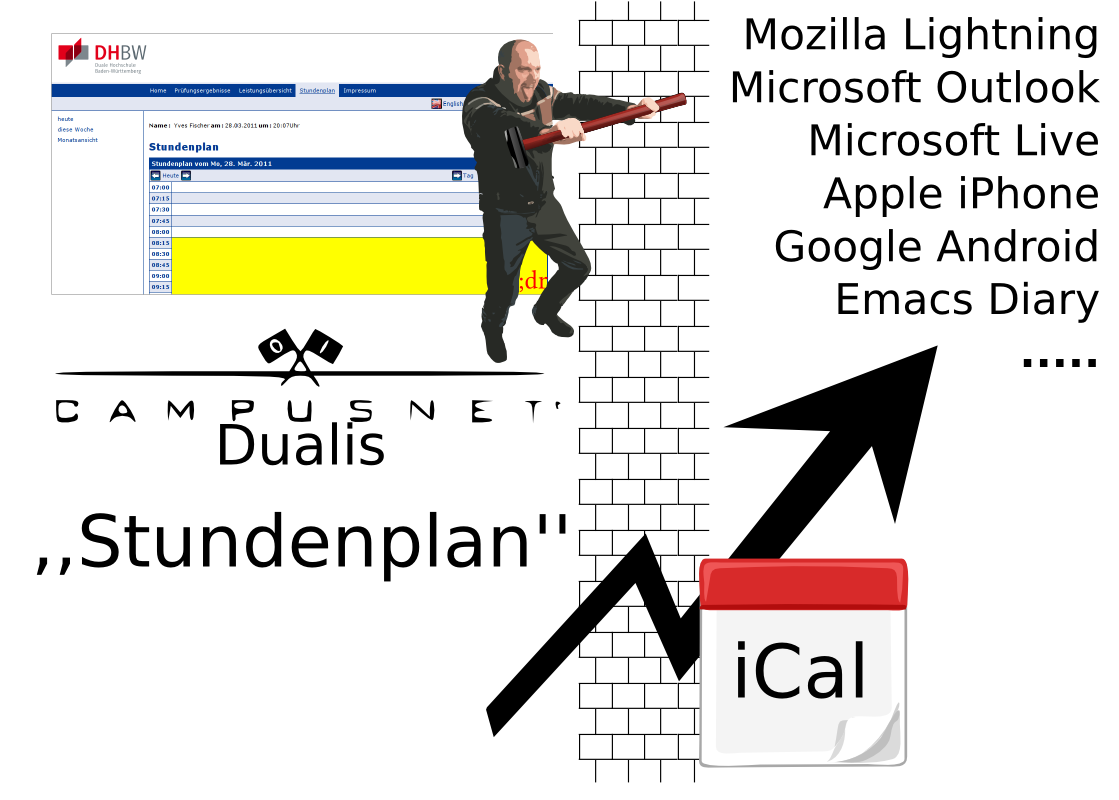
\includegraphics[width=0.9\paperwidth]{images/overview-slide.png}
\end{frame}

\section{Implementierung}
\begin{frame}\frametitle{Mögliche Schnittstellen}
  \begin{itemize}
  \item Apple iPhone
    \begin{itemize}
    \item Direkte iCalendar/HTTPS Unterstützung.
    \end{itemize}
  \item Google Kalender
    \begin{itemize}
    \item schliesst Android Smartphone ein.
    \item Unterstützt Abfragen externer iCalendar/HTTPS Ressourcen.
    \end{itemize}
  \item Mozilla Thunderbird/Lightning
    \begin{itemize}
    \item Direkte iCalendar/HTTPS Unterstützung.
    \end{itemize}
  \item Microsoft Outlook
    \begin{itemize}
    \item Direkte iCalendar/HTTPS Unterstützung.
    \end{itemize}
  \item Microsoft Windows Live
    \begin{itemize}
    \item schliesst Windows Mail, Windows Mobile ein.
    \item beschränkt Abfragen von iCalendar/HTTP Resourcen.
    \end{itemize}
    \pause
  \item \textsc{DUALIS}
    \begin{itemize}
    \item soweit keine zugänglichen Schnittstellen bekannt.
    \end{itemize}
  \end{itemize}
\end{frame}

\begin{frame}\frametitle{Architektur}
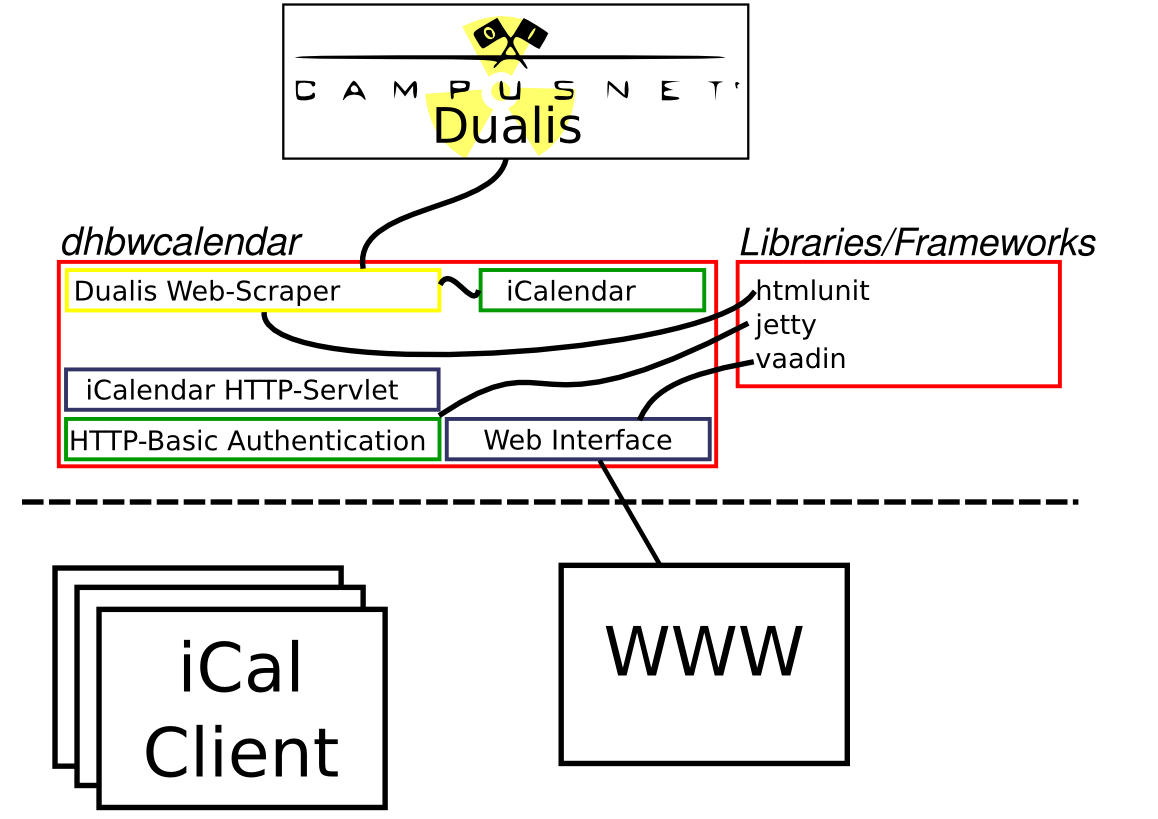
\includegraphics[width=0.8\paperwidth]{images/arch.png}
\end{frame}

\section{Screenshots}
\begin{frame}\frametitle{Apple iPhone}
  \begin{figure}
    \centering
    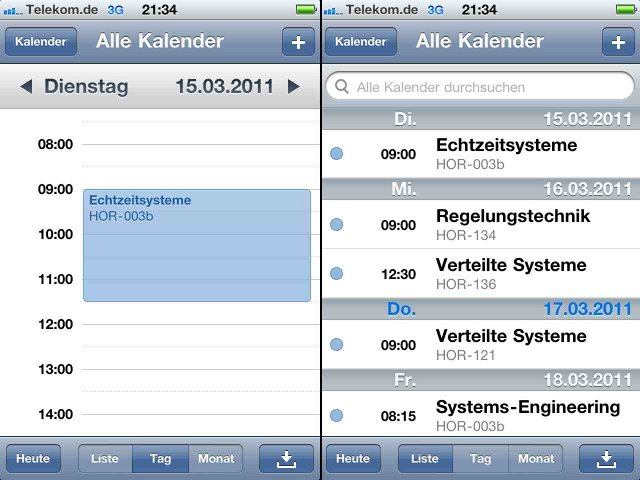
\includegraphics[height=0.6\paperheight]{images/dhbwcalendar-iphone.jpg}
  \end{figure}
  \begin{itemize}
    \item Direkte iCalendar Unterstützung.
  \end{itemize}
\end{frame}

\begin{frame}\frametitle{Google Kalender}
  \begin{figure}
    \centering
    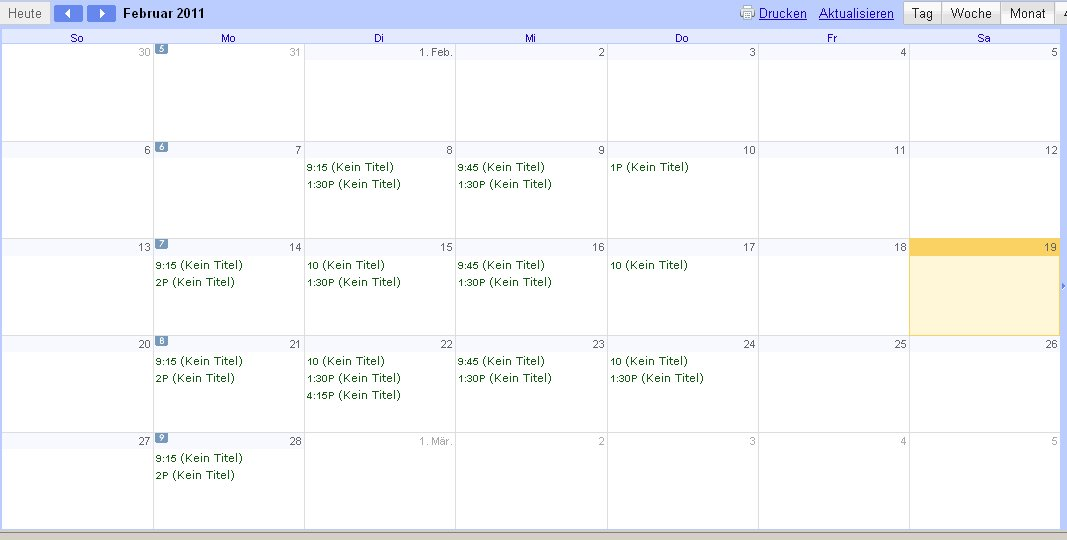
\includegraphics[height=0.5\paperheight]{images/dhbwcalendar-google.jpg}
  \end{figure}
  \begin{itemize}
    \item Unterstützt Abfragen externer iCalendar Ressourcen.
  \end{itemize}
\end{frame}

\begin{frame}\frametitle{Android Smartphones}
  \begin{figure}
    \centering
    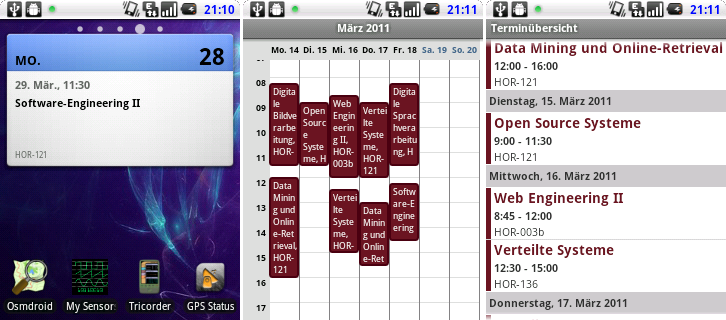
\includegraphics[height=0.5\paperheight]{images/dhbwcalendar-android.png}
  \end{figure}
  \begin{itemize}
    \item Über Synchronisation mit Google Kalender.
  \end{itemize}
\end{frame}

\begin{frame}\frametitle{Outlook 2007}
  \begin{figure}
    \centering
    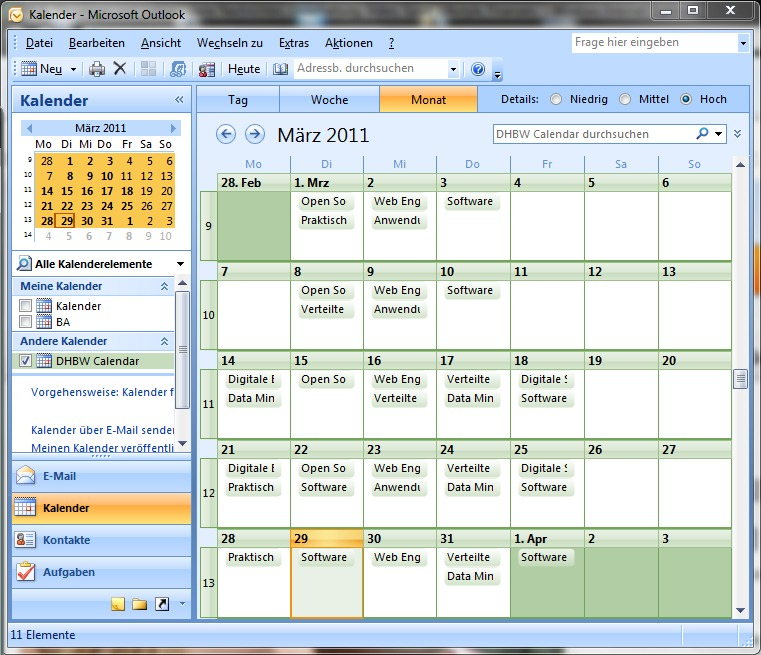
\includegraphics[height=0.6\paperheight]{images/dhbwcalendar-outlook2007.jpg}
  \end{figure}
  \begin{itemize}
    \item Unterstützt Abfragen externer iCalendar Ressourcen.
  \end{itemize}
\end{frame}

\begin{frame}\frametitle{Windows Live}
  \begin{figure}
    \centering
    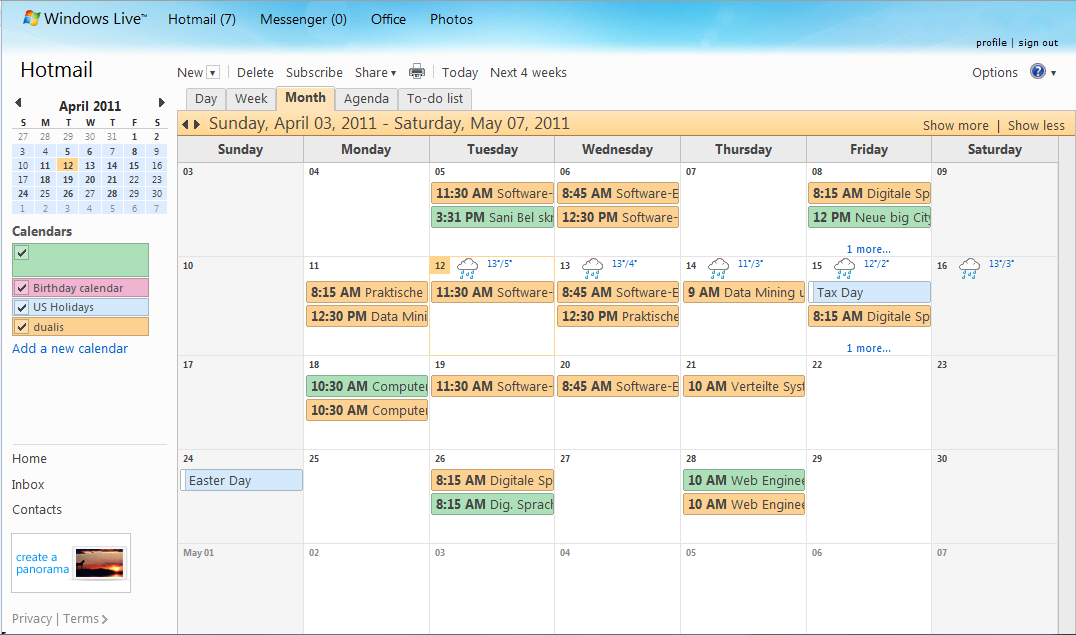
\includegraphics[height=0.6\paperheight]{images/dhbwcalendar-live-web.png}
  \end{figure}
  \begin{itemize}
    \item Unterstützt kein SSL
    \item Unterstützt keine HTTP-Authentifizierung
    \item Workaround: Credentials in Query-String der URL
  \end{itemize}
\end{frame}

\begin{frame}\frametitle{Windows Mail}
  \begin{figure}
    \centering
    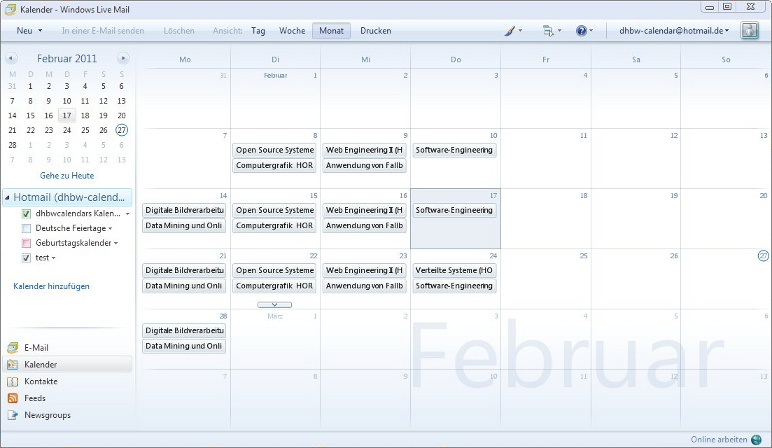
\includegraphics[height=0.6\paperheight]{images/dhbwcalendar-live-desktop.jpg}
  \end{figure}
  \begin{itemize}
    \item Über Synchronisation mit Windows Live.
  \end{itemize}
\end{frame}

\begin{frame}\frametitle{Windows Mobile}
  \visible<1->{
    \begin{itemize}
    \item Theoretisch über Synchronisation mit Windows Live.
    \item Aber nur für den primären Kalender
    \item siehe \url{http://support.microsoft.com/kb/2430181/de}
    \end{itemize}
  }
  \vspace{1cm}
  \visible<2->{
    \begin{center}
      {\huge \tt \#fail}
    \end{center}
  }
\end{frame}

\begin{frame}\frametitle{Mozilla Thunderbird+Lightning}
  \begin{figure}
    \centering
    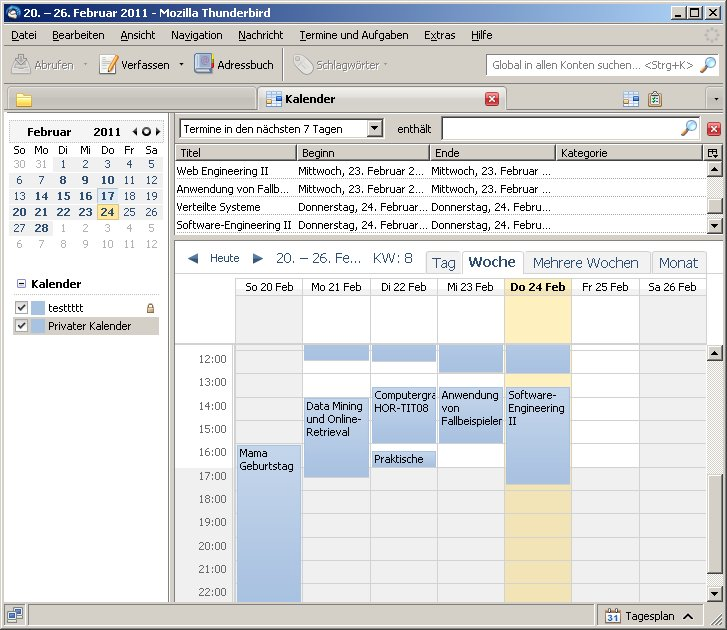
\includegraphics[height=0.6\paperheight]{images/dhbwcalendar-lightning.jpg}
  \end{figure}
  \begin{itemize}
    \item Direkte iCalendar Unterstützung.
  \end{itemize}
\end{frame}


\section{Projekt}

\begin{frame}\frametitle{Open-Source Projekt}
  \begin{itemize}
  \item Java Projekt mit Apache-maven als Werkzeug
  \item Github Hosting für
    \begin{itemize}
    \item Code
    \item Issues
    \item Projektwebsite \url{http://dhbw-horb.github.com/dhbw-calendar}
    \end{itemize}
  \item Projektwebsite mit maven generiert:
    \begin{itemize}
      \item Java-Docs
      \item Dependencies Report
      \item Benutzeranleitung
      \item Dokumentation
    \end{itemize}
  \end{itemize}
\end{frame}


\begin{frame}
\begin{center}
  \huge ------ \\
  \url{http://dhbw-horb.github.com/dhbw-calendar}
\end{center}
\end{frame}

%% \appendix
%% %\section{Schrottfolien}
%% \frame{\begin{center}\huge Schrottfolien\end{center}}
%% \begin{frame}
%% \end{frame}
%% \begin{frame}
%% \end{frame}
\end{document}
